\chapter{Requirements and Technical Study (Sprint 0)}

\section{Introduction}

Before implementation began, a detailed analysis phase was conducted to identify functional needs, define technical architecture, and prepare the development environment. This phase, referred to as \textbf{Sprint 0}, laid the foundation for the subsequent iterative sprints and ensured that the project was aligned with both business objectives and technical constraints.

\section{Identification of Requirements}

\subsection{Actors and User Roles}

The system defines two distinct roles:

\begin{itemize}
  \item \textbf{Cashier}: Executes sales operations, adds products to the cart, processes payments, and generates invoices.
  \item \textbf{Administrator}: Manages product inventory, updates stock, and visualizes sales data through analytics dashboards.
\end{itemize}

\subsection{Functional Requirements}

\begin{itemize}
  \item Login interface with secure authentication.
  \item Role-based redirection to either POS or admin dashboard.
  \item Product browsing with dynamic cart system.
  \item Invoice generation with QR code.
  \item Admin interface for product and stock management.
  \item Embedded analytics dashboards for real-time insights.
\end{itemize}

\subsection{Non-Functional Requirements}

\begin{itemize}
  \item Responsive design for desktop and tablet devices.
  \item Secure access with role-based control.
  \item Fast data fetching and UI rendering.
  \item Clean and intuitive user interface.
\end{itemize}

\subsection{Decision-Oriented Requirements}

\begin{itemize}
  \item Power BI integration for sales trends and product performance.
  \item Ability to view top-selling items and total revenue per user.
  \item Dashboard embedded directly in admin panel.
\end{itemize}

\section{Scrum Planning and Project Setup}

\subsection{Team Structure}

Although the internship was individual, the Scrum methodology was simulated with the following roles:

\begin{itemize}
  \item \textbf{Developer (intern)}: Handles the entire software development lifecycle.
  \item \textbf{Professional Supervisor}: Guides technical decisions and validates deliverables.
  \item \textbf{Academic Supervisor}: Follows academic progression and report quality.
\end{itemize}

\subsection{Sprint 0 Objectives}

\begin{itemize}
  \item Define user stories and identify actors.
  \item Specify system features.
  \item Design global use case diagram.
  \item Set up development tools and repository.
  \item Choose technology stack and define architecture.
\end{itemize}

\section{Use Case Analysis}

The POS system was designed to accommodate two primary user roles with specific permissions and capabilities. The following use case analysis identifies the interactions between system users and the application's core features.

\begin{figure}[H]
  \centering
  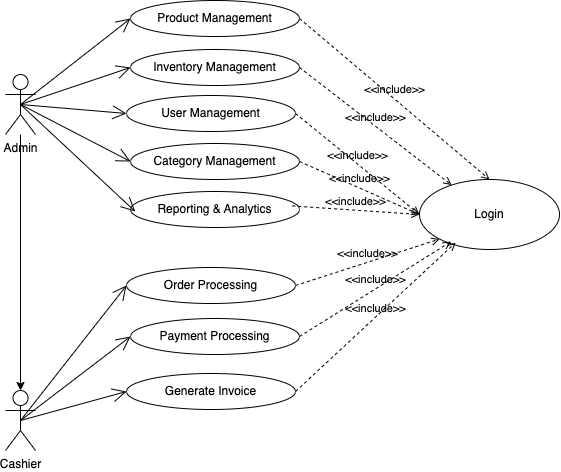
\includegraphics[width=0.9\textwidth]{figures/images/sprint0usecase.png}
  \caption{Global Use Case Diagram – POS System Overview}
  \label{fig:sprint0-usecase}
\end{figure}

\subsection*{Admin User Use Cases}
\begin{itemize}
  \item Access analytics dashboard and embedded Power BI reports
  \item Manage products: create, edit, delete, and update inventory
  \item View sales data and transaction history
  \item Configure system settings and user permissions
  \item Generate reports and export data
\end{itemize}

\subsection*{Cashier User Use Cases}
\begin{itemize}
  \item Login with secure authentication
  \item Browse products and view product details
  \item Add products to cart and manage quantities
  \item Process payments and complete transactions
  \item Generate and print invoices with QR codes
  \item View basic transaction history
\end{itemize}

\section{Technical Environment}

\subsection{Project Methodology – Scrum}

The Scrum framework was used to manage the project across five iterative sprints. Each sprint lasted approximately one week and included planning, execution, testing, and review.

\textbf{Scrum Sprint Structure:}
\begin{itemize}
  \item Sprint 0 – Planning and environment setup
  \item Sprint 1 – Authentication and role management
  \item Sprint 2 – POS dashboard and cart logic
  \item Sprint 3 – Invoicing and stock updates
  \item Sprint 4 – Analytics dashboard with Power BI
\end{itemize}

\subsection{Tools and Technologies Used}

\subsubsection*{React {1}}
\begin{figure}[H]
  \centering
  
\includegraphics[width=0.25\textwidth]{figures/logos/react-logo.png}
  \caption{React Logo}
\end{figure}
React is a JavaScript library for building user interfaces. It powered the cashier/admin dashboards and rendered dynamic views.

\subsubsection*{Next.js {2}}
\begin{figure}[H]
  \centering
  
\includegraphics[width=0.25\textwidth]{figures/logos/nextjs-logo.png}
  \caption{Next.js Logo}
\end{figure}
Next.js served as the fullstack framework, providing routing, backend API endpoints, and deployment support.

\subsubsection*{Tailwind CSS {3}}
\begin{figure}[H]
  \centering
  
\includegraphics[width=0.25\textwidth]{figures/logos/tailwind-logo.png}
  \caption{Tailwind CSS Logo}
\end{figure}
Tailwind CSS was used for UI styling and responsiveness across devices.

\subsubsection*{PostgreSQL {4}}
\begin{figure}[H]
  \centering
  
\includegraphics[width=0.25\textwidth]{figures/logos/postgresql-logo.png}
  \caption{PostgreSQL Logo}
\end{figure}
PostgreSQL stored user, product, invoice, and transaction data.

\subsubsection*{Power BI {5}}
\begin{figure}[H]
  \centering
  
\includegraphics[width=0.25\textwidth]{figures/logos/powerbi-logo.png}
  \caption{Power BI Logo}
\end{figure}
Power BI dashboards were embedded into the admin panel for live decision-making.

\subsubsection*{Auth0 {6}}
\begin{figure}[H]
  \centering
  
\includegraphics[width=0.25\textwidth]{figures/logos/auth0-logo.png}
  \caption{Auth0 Logo}
\end{figure}
Auth0 handled secure login, session management, and access control.

\subsubsection*{Visual Studio Code {7}}
\begin{figure}[H]
  \centering
  
\includegraphics[width=0.25\textwidth]{figures/logos/vscode-logo.png}
  \caption{Visual Studio Code Logo}
\end{figure}
VS Code was the main IDE used for development and debugging.

\subsubsection*{PlantUML {8}}
\begin{figure}[H]
  \centering
  
\includegraphics[width=0.25\textwidth]{figures/logos/uml-logo.png}
  \caption{PlantUML Logo}
\end{figure}
PlantUML generated all UML diagrams used in the documentation.

\subsection{Tool Summary Table}

\begin{table}[H]
\centering
\begin{tabular}{|c|c|p{8cm}|}
\hline
\textbf{Logo} & \textbf{Tool Name} & \textbf{Purpose / Use Case} \\
\hline

\includegraphics[width=0.08\textwidth]{figures/logos/vscode-logo.png} & VS Code {7} & Source code editing and development \\
\hline

\includegraphics[width=0.08\textwidth]{figures/logos/react-logo.png} & React {1} & Frontend UI for POS and admin \\
\hline

\includegraphics[width=0.08\textwidth]{figures/logos/nextjs-logo.png} & Next.js {2} & Fullstack framework and API \\
\hline

\includegraphics[width=0.08\textwidth]{figures/logos/tailwind-logo.png} & Tailwind CSS {3} & UI styling and responsive design \\
\hline

\includegraphics[width=0.08\textwidth]{figures/logos/postgresql-logo.png} & PostgreSQL {4} & Database for products and invoices \\
\hline

\includegraphics[width=0.08\textwidth]{figures/logos/powerbi-logo.png} & Power BI {5} & Embedded analytics dashboards \\
\hline

\includegraphics[width=0.08\textwidth]{figures/logos/auth0-logo.png} & Auth0 {6} & Secure login and role routing \\
\hline

\includegraphics[width=0.08\textwidth]{figures/logos/uml-logo.png} & PlantUML {8} & UML diagram generation \\
\hline
\end{tabular}
\caption{Summary of Technologies and Tools}
\label{tab:tools-summary}
\end{table}

\subsection{System Architecture Overview}

\begin{figure}[H]
  \centering
  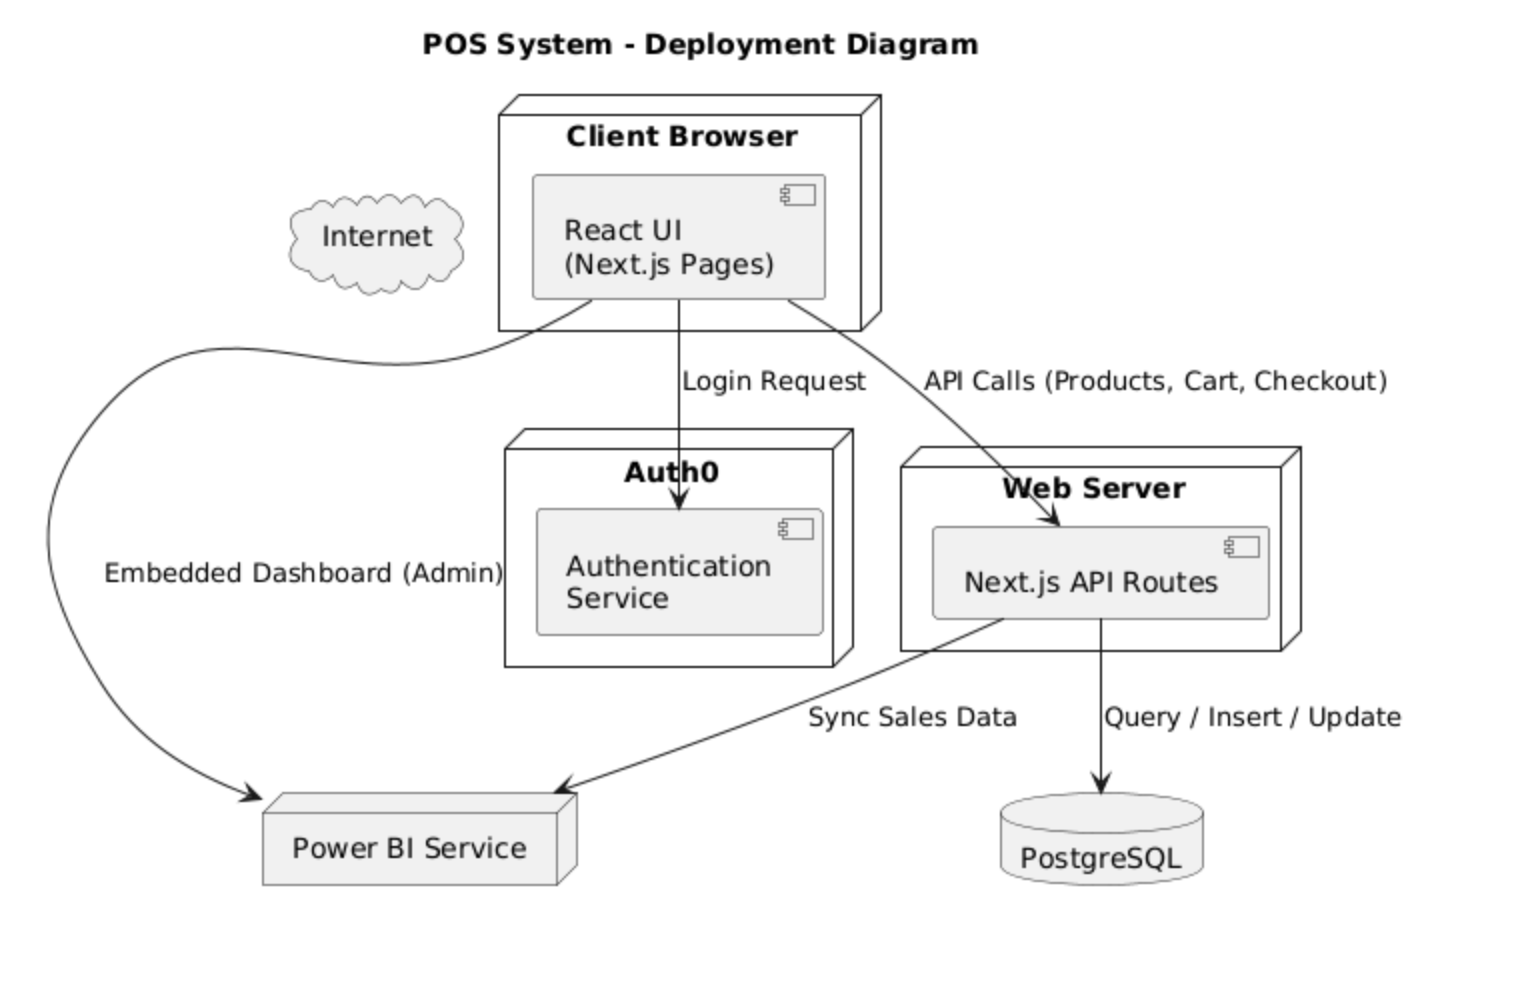
\includegraphics[width=0.9\textwidth]{figures/images/sprint0deployment.png}
  \caption{System Deployment Architecture – POS System Infrastructure}
  \label{fig:sprint0-deployment}
\end{figure}

The architecture demonstrates:

\begin{itemize}
  \item \textbf{Frontend Layer:} React and Tailwind CSS in a Next.js app.
  \item \textbf{Backend Layer:} Next.js API routes with database access.
  \item \textbf{Authentication Layer:} Auth0 for secure login and role-based redirection.
  \item \textbf{Analytics Layer:} Embedded Power BI dashboard for admins.
\end{itemize}

\subsection{System Class Overview}

\begin{figure}[H]
  \centering
  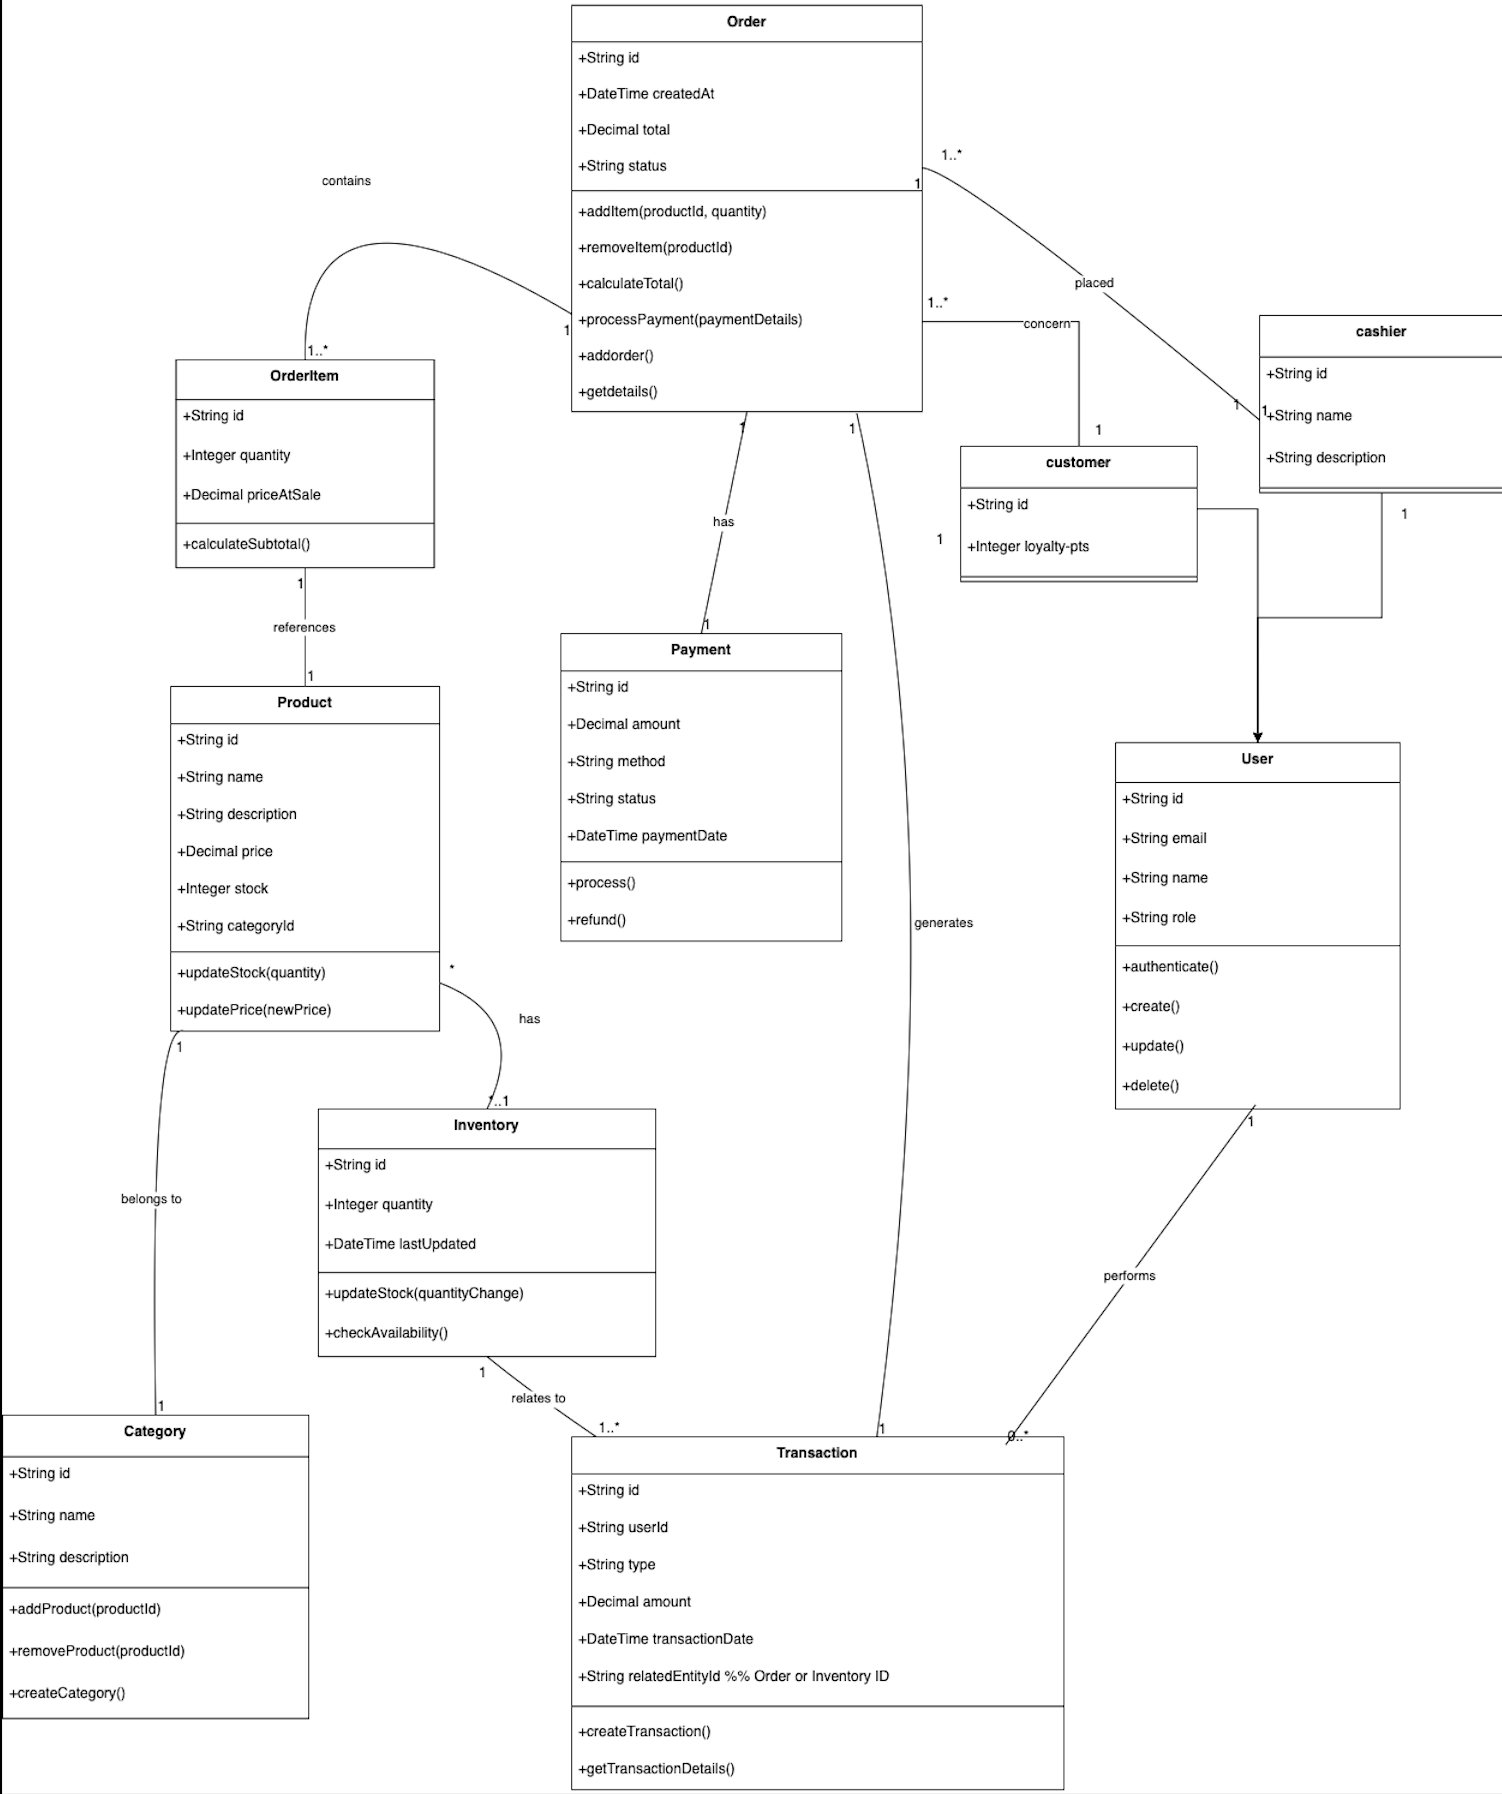
\includegraphics[width=0.9\textwidth]{figures/images/sprint0class.png}
  \caption{Sprint 0 – System Class Diagram}
  \label{fig:sprint0-class}
\end{figure}

\section{Conclusion}

Sprint 0 helped define the project's direction by identifying user roles, and setting up the full technical environment. This foundation allowed the development phase to proceed in sprints, each targeting a functional milestone. The next chapter details the work carried out in Sprint 1: user authentication and secure role-based redirection.